\documentclass[10pt]{article}
\usepackage[a4paper,landscape,margin=14mm]{geometry}
\usepackage[T1]{fontenc}
\usepackage{lmodern}
\usepackage{pgfplots}
\pgfplotsset{compat=1.18}
\definecolor{rlBlue}{HTML}{0072B2}
\definecolor{rlOrange}{HTML}{D55E00}
\definecolor{rlGreen}{HTML}{009E73}
% Generated from the verified job 5047137 archive; do not edit.
\newcommand{\rlCompCopy}{401.2}
\newcommand{\rlCompTriad}{411.4}
\newcommand{\rlCompGemm}{2448}
\newcommand{\rlCompLaggedTime}{6.50}
\newcommand{\rlCompSpmvTime}{19.37}
\newcommand{\rlCompSpeedup}{2.98}
\newcommand{\rlCompWorkRatio}{1.82}
\newcommand{\rlCompRateRatio}{5.44}

\pagestyle{empty}
\setlength{\parindent}{0pt}
\begin{document}
{\Large\bfseries Empirical counter-based roofline}\hfill Companion to the packed-mesh paper
\par\smallskip
Grace CPU, job 5047137, \texttt{nid006550}: 72 threads, $n=128$, pack size 1024.
FP64 affine interior operators; Rhie--Chow on; cached state gradients; worker THP disabled.
\par\medskip
\begin{minipage}[t]{0.485\textwidth}
  \vspace{0pt}
  % Generated from the verified job 5047137 archive; do not edit.

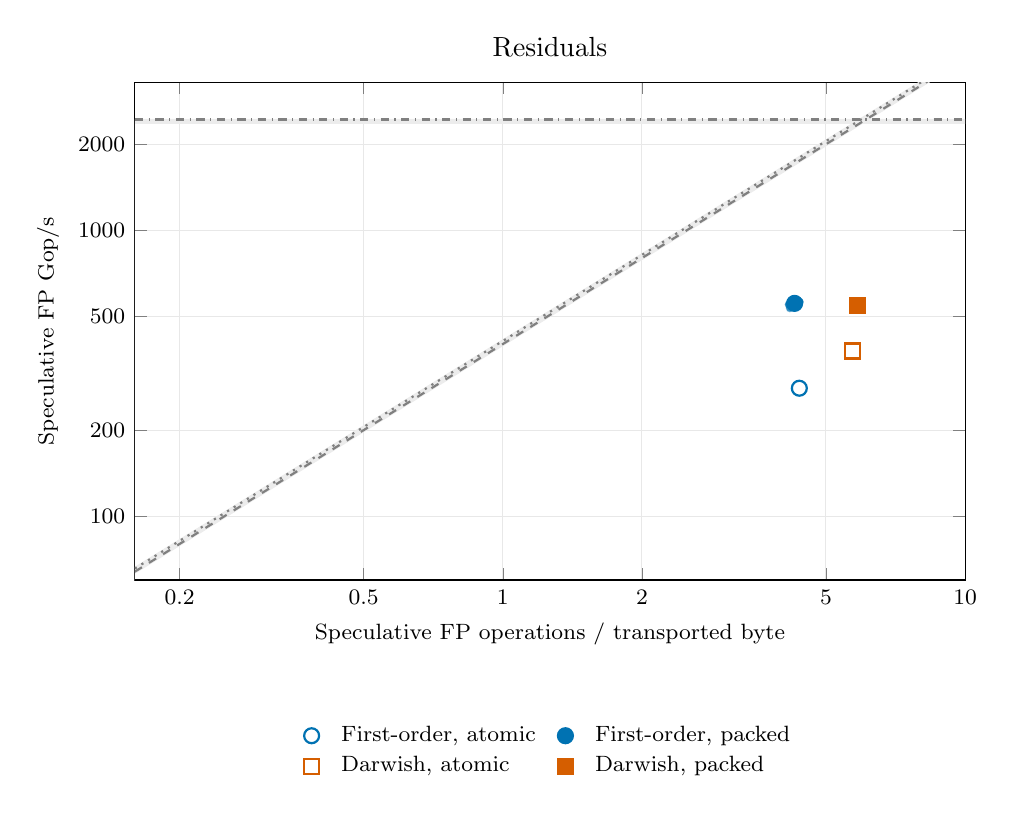
\begin{tikzpicture}
\begin{axis}[
width=\linewidth,height=7.9cm,scale only axis=false,
xmode=log,ymode=log,log basis x=10,log basis y=10,
xmin=0.16,xmax=10,ymin=60,ymax=3300,
xtick={0.2,0.5,1,2,5,10},xticklabels={0.2,0.5,1,2,5,10},
ytick={100,200,500,1000,2000},yticklabels={100,200,500,1000,2000},
xlabel={Speculative FP operations / transported byte},
ylabel={Speculative FP Gop/s},title={Residuals},
grid=major,major grid style={gray!18},tick label style={font=\footnotesize},
label style={font=\footnotesize},legend columns=2,
legend style={at={(0.5,-0.27)},anchor=north,draw=none,font=\footnotesize,
cells={anchor=west},column sep=6pt},]
\addplot[draw=none,fill=gray!15,forget plot] coordinates {(.16,63.06447108784885) (10,3941.5294429905534) (10,4175.386846696572) (.16,66.80618954714517)} \closedcycle;
\addplot[draw=none,fill=gray!15,forget plot] coordinates {(.16,2363.490814540799) (10,2363.490814540799) (10,2462.050629226856) (.16,2462.050629226856)} \closedcycle;
\addplot[gray,dashed,thick,no marks,forget plot] coordinates {(.16,64.1951897291501) (10,4012.199358071881)};
\addplot[gray,dotted,thick,no marks,forget plot] coordinates {(.16,65.82876003382617) (10,4114.297502114136)};
\addplot[gray,dashdotted,thick,no marks,forget plot] coordinates {(.16,2448.1093146161065) (10,2448.1093146161065)};
\addplot[only marks,color=rlBlue,mark=*,mark options={fill=white},mark size=1.25pt,opacity=0.45,forget plot] coordinates {(4.40018536339,283.343737204) (4.37676714375,281.922865423) (4.37033853198,282.040888282) (4.38620794682,282.093557482) (4.36808772194,281.458045046) (4.369080131,281.712590582) (4.3878325883,272.825823352) (4.40478861035,281.168380445) (4.38412958822,281.019936887) (4.38232509338,281.085635739) (4.37374018746,281.438551702) (4.39846757755,282.70871921) (4.36488821831,282.254140987) (4.38834158634,281.770056427) (4.37086674552,279.093331963) (4.36271392914,282.197810361) (4.36681184214,281.859024975) (4.38673092065,281.505203775)};
\addplot[only marks,color=rlBlue,mark=*,mark options={fill=white},mark size=2.7pt,thick] coordinates {(4.38012798479,281.194349991)};
\addlegendentry{First-order, atomic}
\addplot[only marks,color=rlBlue,mark=*,mark options={fill=rlBlue},mark size=1.25pt,opacity=0.45,forget plot] coordinates {(4.2200106412,557.18335758) (4.20447034295,559.664051847) (4.19818242624,557.139860174) (4.38382631915,564.546092162) (4.35637492148,556.537379226) (4.36225294901,562.62332882) (4.37485175602,564.720149596) (4.38948846149,563.020415796) (4.36860042763,562.422009358) (4.15943399832,552.542555907) (4.15362285814,551.3161423) (4.18388720321,554.229838604) (4.34695795846,564.759766861) (4.37204978986,564.204630316) (4.35431540545,565.492013096) (4.18338596725,539.224072325) (4.1783214948,535.332236273) (4.2094741009,550.541780639)};
\addplot[only marks,color=rlBlue,mark=*,mark options={fill=rlBlue},mark size=2.7pt,thick] coordinates {(4.27775039009,556.972204493)};
\addlegendentry{First-order, packed}
\addplot[only marks,color=rlOrange,mark=square*,mark options={fill=white},mark size=1.25pt,opacity=0.45,forget plot] coordinates {(5.73470476404,379.890858322) (5.71360719056,377.00695415) (5.71654552308,381.854049247) (5.75165379993,379.195673448) (5.73043963625,381.236908695) (5.73566362016,381.583260283) (5.70720350542,374.650039686) (5.70981476921,372.463473117) (5.70061260677,378.111011134) (5.69659990734,382.32794296) (5.6942149302,382.499270135) (5.71491962544,380.183364629) (5.6949033619,381.454602799) (5.72203348171,382.753060376) (5.70421713702,381.750831276) (5.70014570059,377.647873598) (5.70510582697,376.073413182) (5.73004091494,382.620743769)};
\addplot[only marks,color=rlOrange,mark=square*,mark options={fill=white},mark size=2.7pt,thick] coordinates {(5.71457923897,379.627962823)};
\addlegendentry{Darwish, atomic}
\addplot[only marks,color=rlOrange,mark=square*,mark options={fill=rlOrange},mark size=1.25pt,opacity=0.45,forget plot] coordinates {(5.93771876903,528.371343502) (5.88656363653,548.86941674) (5.87926460685,530.777502259) (5.83293034473,548.937674734) (5.7686717493,546.749593416) (5.77733674538,546.048932866) (5.88021978719,549.891784597) (5.93416150754,550.774974043) (5.86525571704,549.786695161) (5.77150609179,546.064757333) (5.75908813302,548.153873121) (5.82290900318,548.146367625) (5.78307271285,546.176239218) (5.84752770303,545.000025729) (5.7948621455,544.78152529) (5.88473351246,549.234253073) (5.89985085074,549.649562161) (5.94706611825,549.997921254)};
\addplot[only marks,color=rlOrange,mark=square*,mark options={fill=rlOrange},mark size=2.7pt,thick] coordinates {(5.84848550747,545.967357896)};
\addlegendentry{Darwish, packed}
\end{axis}
\end{tikzpicture}

\end{minipage}\hfill
\begin{minipage}[t]{0.485\textwidth}
  \vspace{0pt}
  % Generated from the verified job 5047137 archive; do not edit.

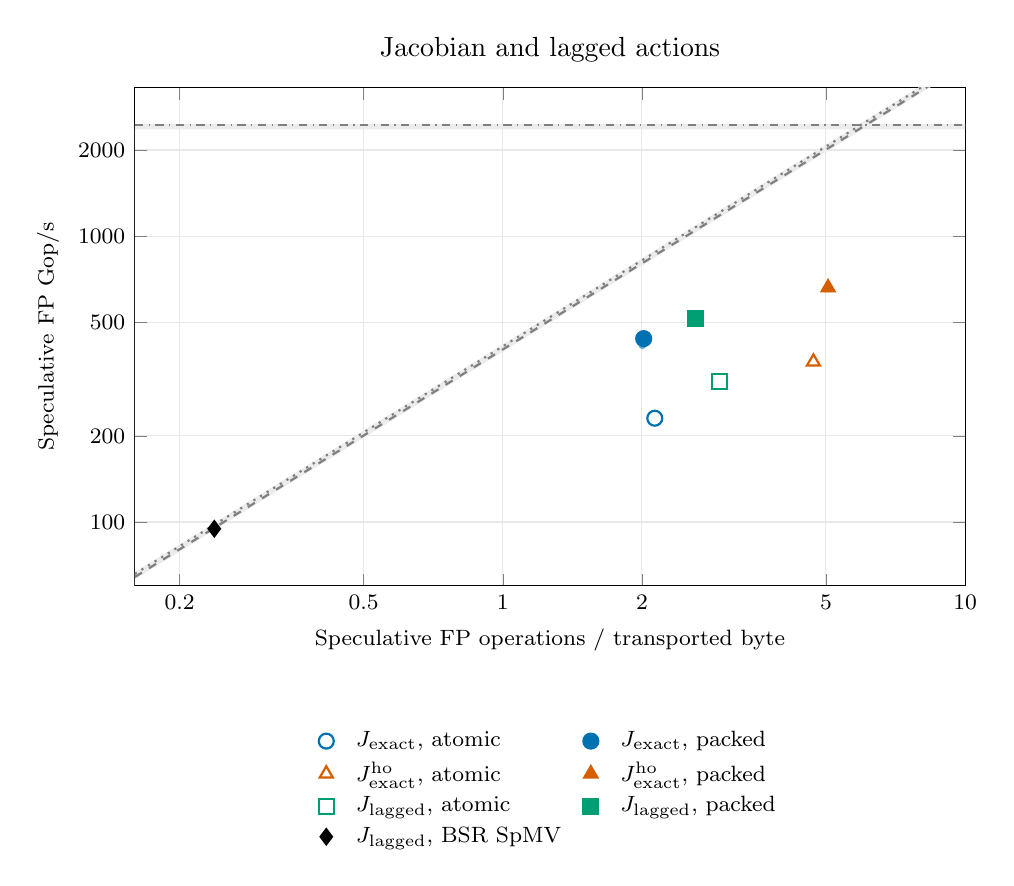
\begin{tikzpicture}
\begin{axis}[
width=\linewidth,height=7.9cm,scale only axis=false,
xmode=log,ymode=log,log basis x=10,log basis y=10,
xmin=0.16,xmax=10,ymin=60,ymax=3300,
xtick={0.2,0.5,1,2,5,10},xticklabels={0.2,0.5,1,2,5,10},
ytick={100,200,500,1000,2000},yticklabels={100,200,500,1000,2000},
xlabel={Speculative FP operations / transported byte},
ylabel={Speculative FP Gop/s},title={Jacobian and lagged actions},
grid=major,major grid style={gray!18},tick label style={font=\footnotesize},
label style={font=\footnotesize},legend columns=2,
legend style={at={(0.5,-0.27)},anchor=north,draw=none,font=\footnotesize,
cells={anchor=west},column sep=6pt},]
\addplot[draw=none,fill=gray!15,forget plot] coordinates {(.16,63.06447108784885) (10,3941.5294429905534) (10,4175.386846696572) (.16,66.80618954714517)} \closedcycle;
\addplot[draw=none,fill=gray!15,forget plot] coordinates {(.16,2363.490814540799) (10,2363.490814540799) (10,2462.050629226856) (.16,2462.050629226856)} \closedcycle;
\addplot[gray,dashed,thick,no marks,forget plot] coordinates {(.16,64.1951897291501) (10,4012.199358071881)};
\addplot[gray,dotted,thick,no marks,forget plot] coordinates {(.16,65.82876003382617) (10,4114.297502114136)};
\addplot[gray,dashdotted,thick,no marks,forget plot] coordinates {(.16,2448.1093146161065) (10,2448.1093146161065)};
\addplot[only marks,color=rlBlue,mark=*,mark options={fill=white},mark size=1.25pt,opacity=0.45,forget plot] coordinates {(2.13207590952,231.873734998) (2.13097435697,228.570551888) (2.12796178765,230.436064991) (2.13562528295,233.214614072) (2.13280643722,232.699417569) (2.13239152046,231.059666712) (2.1317926531,231.472191932) (2.1341755477,228.35069672) (2.13027720151,228.596496762) (2.13162872839,231.359044136) (2.13311653956,228.068844613) (2.135369812,231.918218177) (2.12997171281,230.899017163) (2.13330022813,231.609382154) (2.12907790487,224.732859252) (2.12974139016,231.029795963) (2.13112725537,232.423236102) (2.13440850708,232.940273223)};
\addplot[only marks,color=rlBlue,mark=*,mark options={fill=white},mark size=2.7pt,thick] coordinates {(2.13199015419,230.625228135)};
\addlegendentry{$J_{\rm exact}$, atomic}
\addplot[only marks,color=rlBlue,mark=*,mark options={fill=rlBlue},mark size=1.25pt,opacity=0.45,forget plot] coordinates {(2.01733942707,435.175632297) (2.01319408483,440.873511672) (2.00972444802,437.224904152) (2.01984813349,439.982598411) (2.01191392359,437.816537914) (2.01447899282,439.776793364) (2.01742866746,438.377297052) (2.02446286581,440.657154691) (2.01224177677,438.551810196) (2.01962741606,439.221741231) (2.01521400346,437.624104196) (2.02466296917,439.084385408) (2.0252595409,441.454349017) (2.03286506605,441.728836445) (2.02606007196,441.709081309) (2.00732951641,437.741258251) (2.00519234042,415.215892745) (2.01403113851,439.936715144)};
\addplot[only marks,color=rlBlue,mark=*,mark options={fill=rlBlue},mark size=2.7pt,thick] coordinates {(2.01727079904,437.897366861)};
\addlegendentry{$J_{\rm exact}$, packed}
\addplot[only marks,color=rlOrange,mark=triangle*,mark options={fill=white},mark size=1.25pt,opacity=0.45,forget plot] coordinates {(4.69642261576,364.141565012) (4.69261270229,364.094014482) (4.69089423986,361.65261249) (4.70352895775,360.679020499) (4.69492301472,364.197338891) (4.69451181515,365.132871173) (4.7101669192,364.676269902) (4.7146352799,364.286285891) (4.71041945427,361.223476528) (4.69775163564,361.324498415) (4.69644694165,363.534994909) (4.70098168482,364.187927117) (4.68601252901,364.446843913) (4.68891445449,364.168033161) (4.68454392827,358.51778819) (4.70175690673,363.408428472) (4.69926929511,364.822049888) (4.70259591959,365.116900698)};
\addplot[only marks,color=rlOrange,mark=triangle*,mark options={fill=white},mark size=2.7pt,thick] coordinates {(4.69813268301,363.311717757)};
\addlegendentry{$J^{\rm ho}_{\rm exact}$, atomic}
\addplot[only marks,color=rlOrange,mark=triangle*,mark options={fill=rlOrange},mark size=1.25pt,opacity=0.45,forget plot] coordinates {(5.04110490202,664.124368598) (5.02774323304,655.625753437) (5.03100237986,660.766896763) (5.03617028959,656.953161253) (5.03096758218,655.518401519) (5.03491541632,666.454390073) (5.045280515,663.837865526) (5.04510308702,647.139102329) (5.04601620093,665.216014136) (5.06386280663,657.790968331) (5.06642030559,651.800682139) (5.07263216338,665.879693457) (5.08807848288,666.573021155) (5.09901094857,665.530699716) (5.09110044479,666.561615818) (5.05192020683,656.821219372) (5.05487361453,652.74025726) (5.05941463165,664.00750824)};
\addplot[only marks,color=rlOrange,mark=triangle*,mark options={fill=rlOrange},mark size=2.7pt,thick] coordinates {(5.05475651171,660.185645507)};
\addlegendentry{$J^{\rm ho}_{\rm exact}$, packed}
\addplot[only marks,color=rlGreen,mark=square*,mark options={fill=white},mark size=1.25pt,opacity=0.45,forget plot] coordinates {(2.95852310301,306.752382879) (2.94666135497,311.674620451) (2.93898799806,307.26075111) (2.95954433063,308.824156707) (2.93693522538,311.816409448) (2.94401022323,311.735881531) (2.93506913939,308.626347922) (2.95255653682,310.113289498) (2.92839454789,308.653833602) (2.93740760315,310.746022616) (2.9343659718,311.652962471) (2.95917934048,309.529530241) (2.93695444348,310.152051428) (2.96423078257,312.506424808) (2.94436322536,310.432082313) (2.93304133104,309.265740388) (2.94032299559,310.702676079) (2.95679078739,308.255719087)};
\addplot[only marks,color=rlGreen,mark=square*,mark options={fill=white},mark size=2.7pt,thick] coordinates {(2.94485216335,309.92782681)};
\addlegendentry{$J_{\rm lagged}$, atomic}
\addplot[only marks,color=rlGreen,mark=square*,mark options={fill=rlGreen},mark size=1.25pt,opacity=0.45,forget plot] coordinates {(2.62479650191,517.041712764) (2.60883413374,515.656666432) (2.6019562061,515.424377748) (2.61495819392,516.427058486) (2.59704647229,512.502606072) (2.60402807298,516.397947637) (2.61675271725,510.871847334) (2.63269711604,516.95182536) (2.61123696038,515.819543218) (2.62254671825,514.687032443) (2.61620616253,518.456876521) (2.64039997727,519.810271202) (2.59902571653,505.260923737) (2.61975955576,516.112577866) (2.60051361606,514.84014834) (2.61061751219,513.309933376) (2.61381460671,514.112953761) (2.6322739356,514.229141554)};
\addplot[only marks,color=rlGreen,mark=square*,mark options={fill=rlGreen},mark size=2.7pt,thick] coordinates {(2.61485912086,514.884080214)};
\addlegendentry{$J_{\rm lagged}$, packed}
\addplot[only marks,color=black,mark=diamond*,mark options={fill=black},mark size=1.25pt,opacity=0.45,forget plot] coordinates {(0.237658439362,94.8969409895) (0.237714519311,94.6426881143) (0.237744128823,94.7135848788) (0.237561353478,93.0978918521) (0.237598781443,94.4365648596) (0.237610741165,94.7323388728) (0.237705502239,94.5021570111) (0.23770374573,94.9603994533) (0.237723216882,94.9239332692) (0.237624542542,94.954768309) (0.23767808475,94.8153628727) (0.237703974832,95.2248182334) (0.237647056207,94.2734543686) (0.237635688291,94.7033906661) (0.237645817859,94.9956206073) (0.237564571784,94.7214198918) (0.237598559622,94.754583116) (0.237601300659,94.8818463276)};
\addplot[only marks,color=black,mark=diamond*,mark options={fill=black},mark size=2.7pt,thick] coordinates {(0.237651112499,94.6795424274)};
\addlegendentry{$J_{\rm lagged}$, BSR SpMV}
\end{axis}
\end{tikzpicture}

\end{minipage}
\par\medskip
\textbf{Reading the plot.} Small marks show all 18 counted captures per operator;
large marks show the arithmetic mean of their coordinates. Open marks are atomic;
filled marks are packed, with a black diamond for BSR SpMV. Both panels use the same axes.
No background subtraction or sample removal is applied.
\par\smallskip
\textbf{Measured references, not ceilings.} Dashed and dotted diagonals use copy
(\rlCompCopy{} GB/s) and triad (\rlCompTriad{} GB/s) transported bandwidth.
The dash-dot horizontal uses counted DGEMM (\rlCompGemm{} speculative Gop/s).
Gray bands show the full observed ranges, combining copy and triad for bandwidth;
they are not confidence intervals. Workload-specific instruction costs and
synchronization are not modelled by these lines.
\par\smallskip
\textbf{Throughput is not speedup.} The equivalent packed lagged action takes
\rlCompLaggedTime{} ms versus \rlCompSpmvTime{} ms for BSR SpMV in ordinary execution:
\rlCompSpeedup{}$\times$ faster. Its counted work is \rlCompWorkRatio{}$\times$ larger,
so its \rlCompRateRatio{}$\times$ operation-rate ratio is not the speedup.
Exact Jacobians apply different operators from the lagged matrix.
\par\smallskip
\footnotesize
Reproduction, raw-data provenance and interpretation:
\texttt{wip/paper/reproducibility/README.md}. Generated coordinates:
\texttt{roofline-data.json}. This figure supplies performance context; it does
not identify a hardware bottleneck, a universal efficiency bound or a solver speedup.
\end{document}
